\documentclass{article}
\usepackage{tikz}
\usepackage{adjustbox}

\begin{document}

\begin{adjustbox}{center}
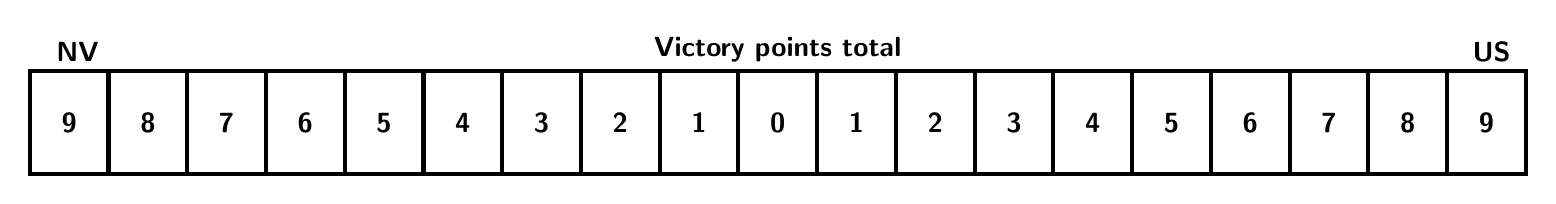
\begin{tikzpicture}
    % Define box size
    \def\boxwidth{1.0}
    \def\boxheight{1.3}
    \def\boxthickness{1.5pt} % Parameterized line thickness

    % Define victory points (NV decreasing, US increasing)
    \def\victorypoints{9, 8, 7, 6, 5, 4, 3, 2, 1, 0, 1, 2, 3, 4, 5, 6, 7, 8, 9}

    \def\ypos{0.25}
    % Labels
    \node[anchor=east] at (1, \ypos) {\sffamily \bfseries NV};
    \node[anchor=west] at (18*\boxwidth + 0.2, \ypos) {\sffamily \bfseries US};
    \node[anchor=south] at (9.5*\boxwidth, \ypos-0.25) {\sffamily \bfseries Victory points total}; % Centered over the track

    % Draw boxes and numbers
    \foreach \x [count=\i] in \victorypoints {
        \pgfmathsetmacro\xpos{\i - 1}
        \draw[line width=\boxthickness] (\xpos*\boxwidth, 0) rectangle (\xpos*\boxwidth + \boxwidth, -\boxheight);
        \node at (\xpos*\boxwidth + 0.5, -0.65) {\sffamily \bfseries \x};
    }

\end{tikzpicture}
\end{adjustbox}

\end{document}
